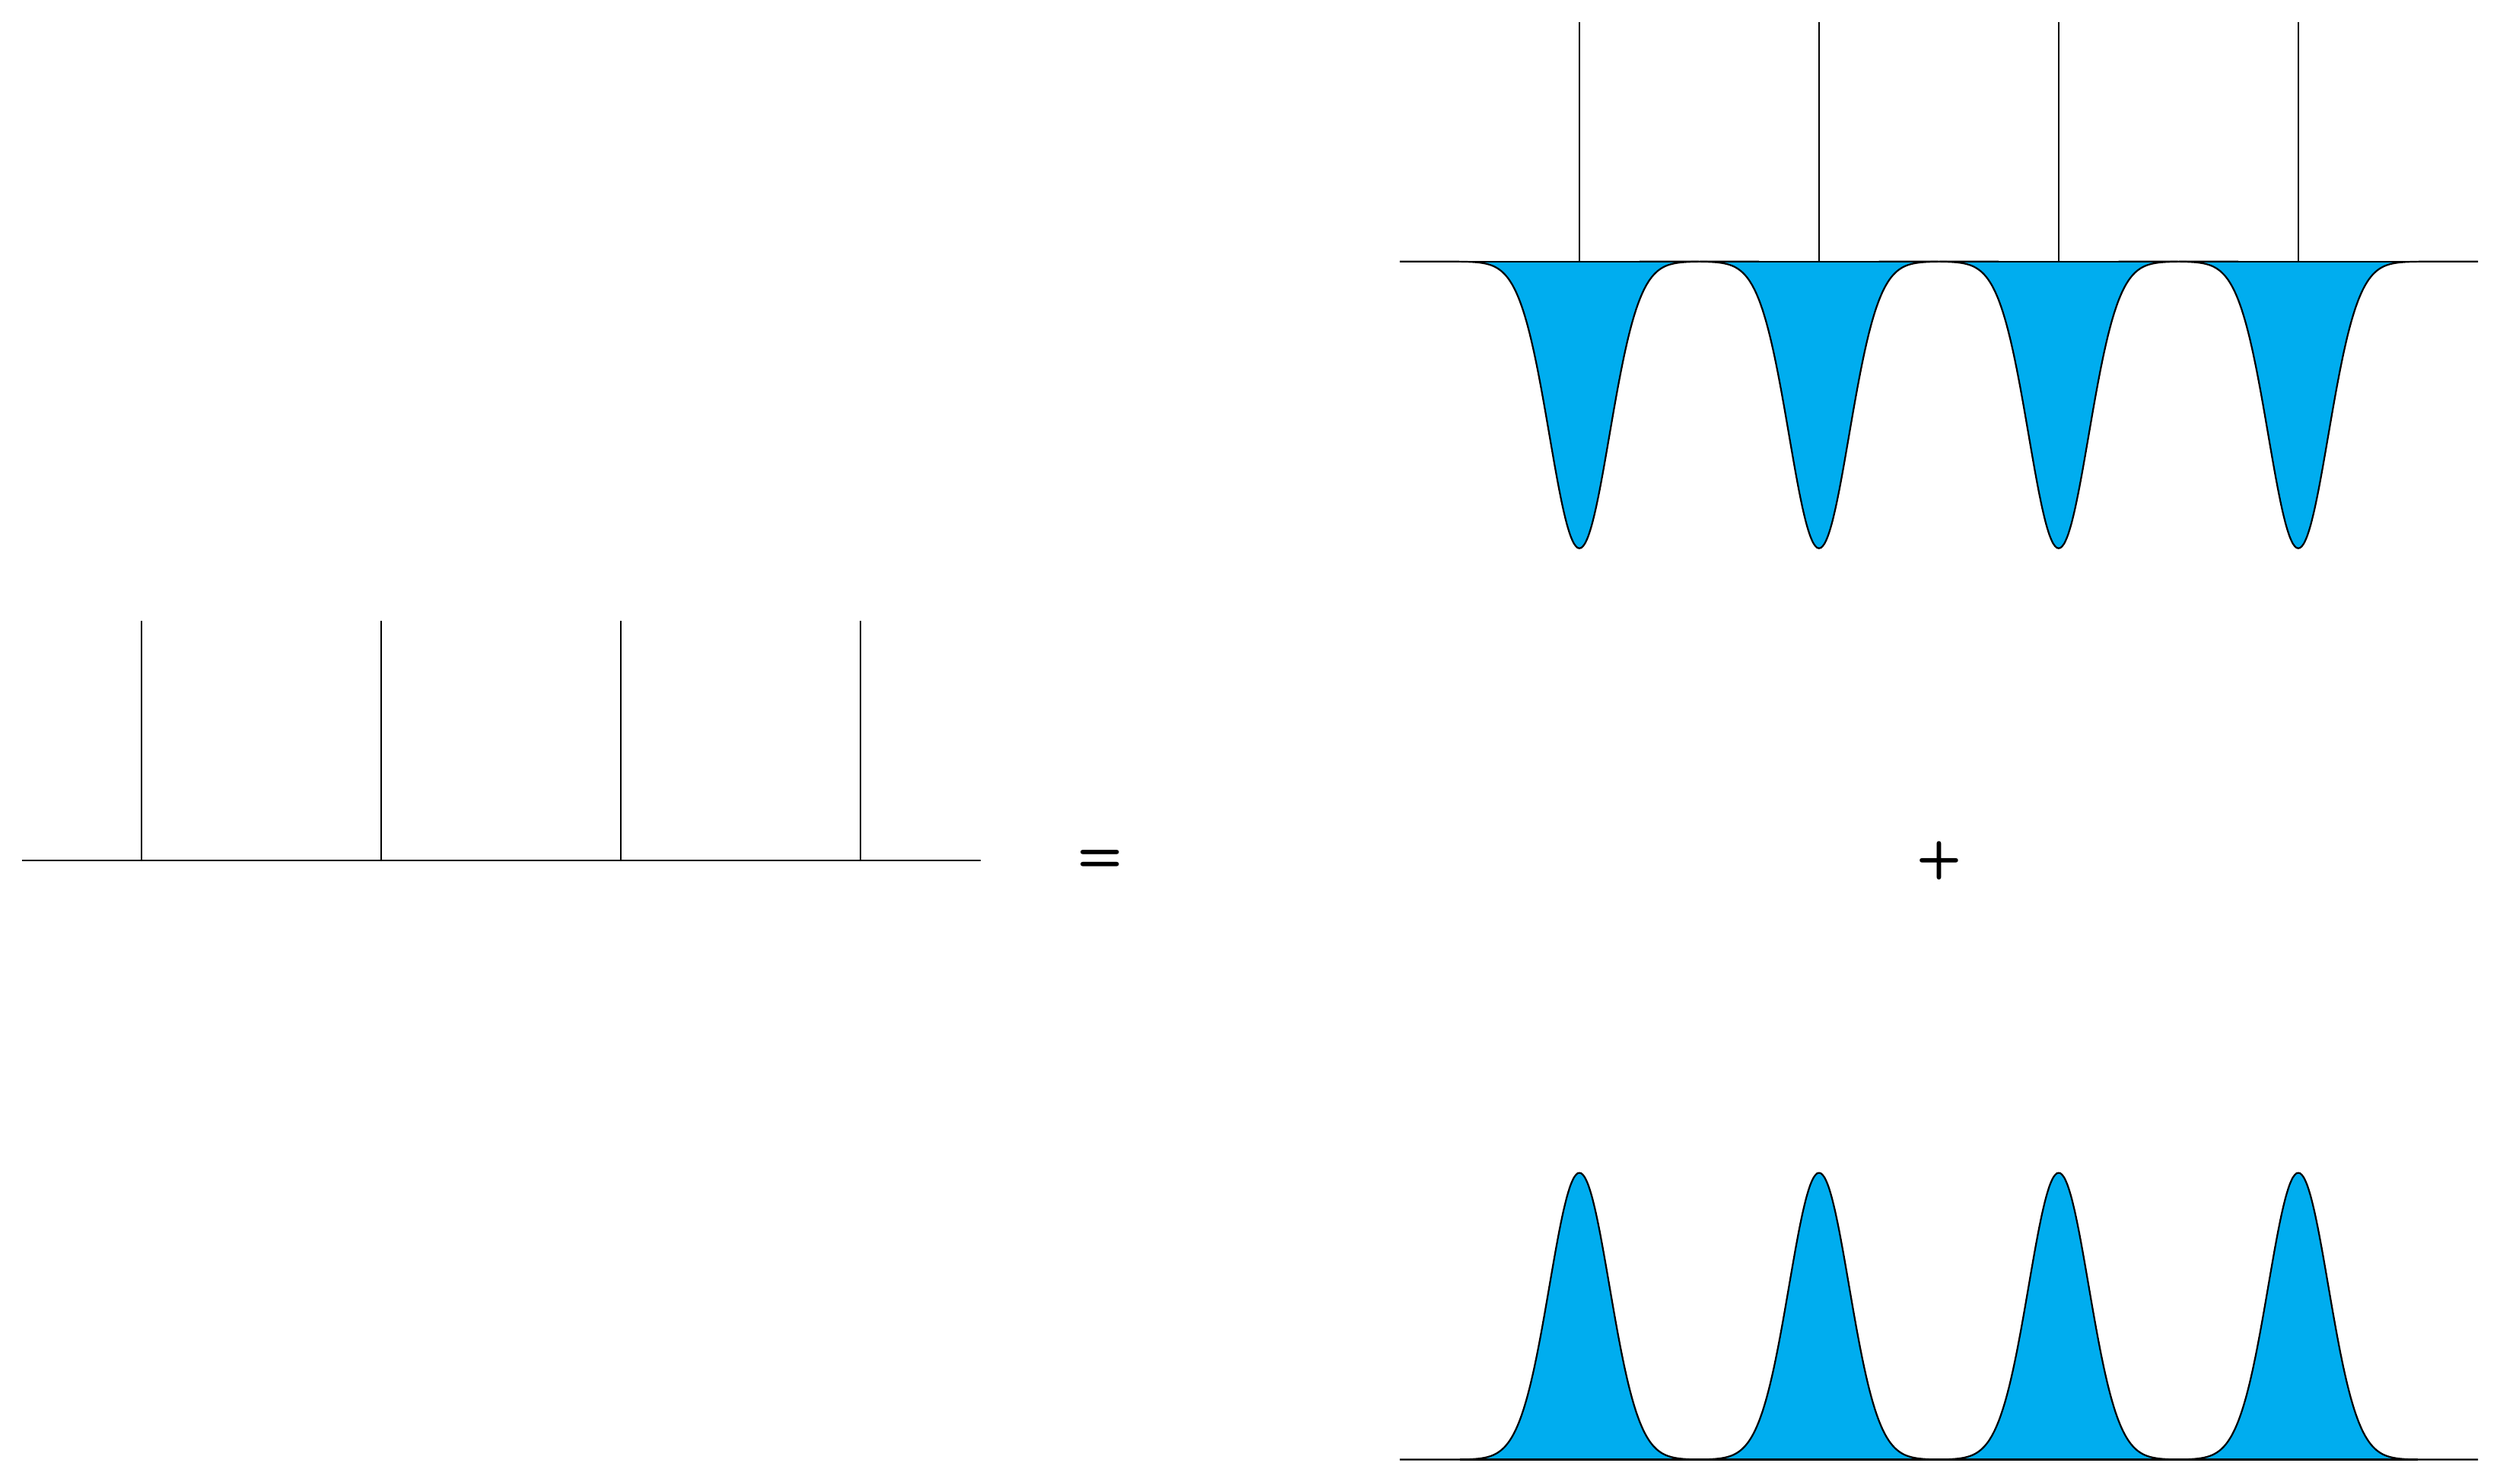
\begin{tikzpicture}
    % First filled Gaussian (centered at -6)
    \fill[cyan] plot[domain=-9:-3, samples=100] 
        ({\x}, {-12/(sqrt(2*pi))*exp(-2*(\x+6)^2)}) -- (-3,0) -- (-9,0) -- cycle;
    \draw[black, thick, smooth] plot[domain=-9:-3, samples=100] 
        ({\x}, {-12/(sqrt(2*pi))*exp(-2*(\x+6)^2)});\
    \draw[black, thick] (-6,0) -- (-6,4);
        
    % Second filled Gaussian (centered at -2)
    \fill[cyan] plot[domain=-5:1, samples=100] 
        ({\x}, {-12/(sqrt(2*pi))*exp(-2*(\x+2)^2)}) -- (1,0) -- (-5,0) -- cycle;
    \draw[black, thick, smooth] plot[domain=-5:1, samples=100] 
        ({\x}, {-12/(sqrt(2*pi))*exp(-2*(\x+2)^2)});
    \draw[black, thick] (-2,0) -- (-2,4);
    
    % Third filled Gaussian (centered at 2)
    \fill[cyan] plot[domain=-1:5, samples=100] 
        ({\x}, {-12/(sqrt(2*pi))*exp(-2*(\x-2)^2)}) -- (5,0) -- (-1,0) -- cycle;
    \draw[black, thick, smooth] plot[domain=-1:5, samples=100] 
        ({\x}, {-12/(sqrt(2*pi))*exp(-2*(\x-2)^2)});
    \draw[black, thick] (2,0) -- (2,4);
    
    % Fourth filled Gaussian (centered at 6)
    \fill[cyan] plot[domain=3:9, samples=100] 
        ({\x}, {-12/(sqrt(2*pi))*exp(-2*(\x-6)^2)}) -- (9,0) -- (3,0) -- cycle;
    \draw[black, thick, smooth] plot[domain=3:9, samples=100] 
        ({\x}, {-12/(sqrt(2*pi))*exp(-2*(\x-6)^2)});
    \draw[black, thick] (6,0) -- (6,4);

    \draw[black, thick] (-8,0) -- (8,0);

    % First filled Gaussian (centered at -6)
    \draw[black, thick] (-30,-10) -- (-30,-6);
        
    % Second filled Gaussian (centered at -2)
    \draw[black, thick] (-26,-10) -- (-26,-6);
    
    % Third filled Gaussian (centered at 2)
    \draw[black, thick] (-22,-10) -- (-22,-6);
    
    % Fourth filled Gaussian (centered at 6)
    \draw[black, thick] (-18,-10) -- (-18,-6);

    \draw[black, thick] (-32,-10) -- (-16,-10);

    \draw (-14,-10) node[font=\fontsize{80}{80}\sffamily\bfseries]{=};

    % First filled Gaussian (centered at -6, shifted downward by 20)
    \fill[cyan] plot[domain=-9:-3, samples=100] 
        ({\x}, {-20 + 12/(sqrt(2*pi))*exp(-2*(\x+6)^2)}) -- (-3,-20) -- (-9,-20) -- cycle;
    \draw[black, thick, smooth] plot[domain=-9:-3, samples=100] 
        ({\x}, {-20 + 12/(sqrt(2*pi))*exp(-2*(\x+6)^2)});
    
    % Second filled Gaussian (centered at -2, shifted downward by 20)
    \fill[cyan] plot[domain=-5:1, samples=100] 
        ({\x}, {-20 + 12/(sqrt(2*pi))*exp(-2*(\x+2)^2)}) -- (1,-20) -- (-5,-20) -- cycle;
    \draw[black, thick, smooth] plot[domain=-5:1, samples=100] 
        ({\x}, {-20 + 12/(sqrt(2*pi))*exp(-2*(\x+2)^2)});
    
    % Third filled Gaussian (centered at 2, shifted downward by 20)
    \fill[cyan] plot[domain=-1:5, samples=100] 
        ({\x}, {-20 + 12/(sqrt(2*pi))*exp(-2*(\x-2)^2)}) -- (5,-20) -- (-1,-20) -- cycle;
    \draw[black, thick, smooth] plot[domain=-1:5, samples=100] 
        ({\x}, {-20 + 12/(sqrt(2*pi))*exp(-2*(\x-2)^2)});
    
    % Fourth filled Gaussian (centered at 6, shifted downward by 20)
    \fill[cyan] plot[domain=3:9, samples=100] 
        ({\x}, {-20 + 12/(sqrt(2*pi))*exp(-2*(\x-6)^2)}) -- (9,-20) -- (3,-20) -- cycle;
    \draw[black, thick, smooth] plot[domain=3:9, samples=100] 
        ({\x}, {-20 + 12/(sqrt(2*pi))*exp(-2*(\x-6)^2)});

    \draw[black, thick] (-8,-20) -- (8,-20);

    \draw (0,-10) node[font=\fontsize{80}{80}\sffamily\bfseries]{+};

\end{tikzpicture}